%So far we have focused on region-wide trends. However, we will now discuss the impacts at a local level for three communities, starting with one travel analysis zone (TAZ) of the downtown financial district of San Francisco (Figure~\ref{fig:equity_study_area}). As mentioned, San Francisco in general is expected to experience less loss in accessibility than most other communities. 
In this section, we will explore some possible explanations for why this San Francisco TAZ (Figure~\ref{fig:equity_study_area}) has lower expected accessibility losses than most other communities.
%something about walking!
First, the financial district of San Francisco differs dramatically from many other TAZs in that the percentage of trips made by car is relatively small (38\% versus an average of 85\% across all TAZs). Households traveling by foot or bike will be less influenced by network damage, because the model considers only damage to the road network and transit systems; thus, foot travel routes and travel times will not be affected in this model. We also observe that more trips by foot and bike correspond to destinations that are closer geographically. The impact of travel mode shift post-earthquake will be further explored in Section~\ref{sec:accDisc}.
 
 % loss exceedance curve. something about they take short trips.
 Second,  Figure~\ref{fig:time_distance_pdfs}{(a)} shows that the average time for a trip to and from work is about average for a TAZ in this region and also follows a similar distribution to that of the other TAZs. Figure~\ref{fig:time_distance_pdfs}{(b)} suggests a slight trend towards shorter trips, but the average trip distance for trips is only 7\% lower than the average for all trips region-wide. Since the trip time and length are relatively typical, but the accessibility is much lower than average, the trip time and length do not explain the differences in accessibility losses.
 
% may play a role in the relative accessibility risk for this TAZ, but other factors or combination of factors are likely more important. 

\begin{figure}
\centering
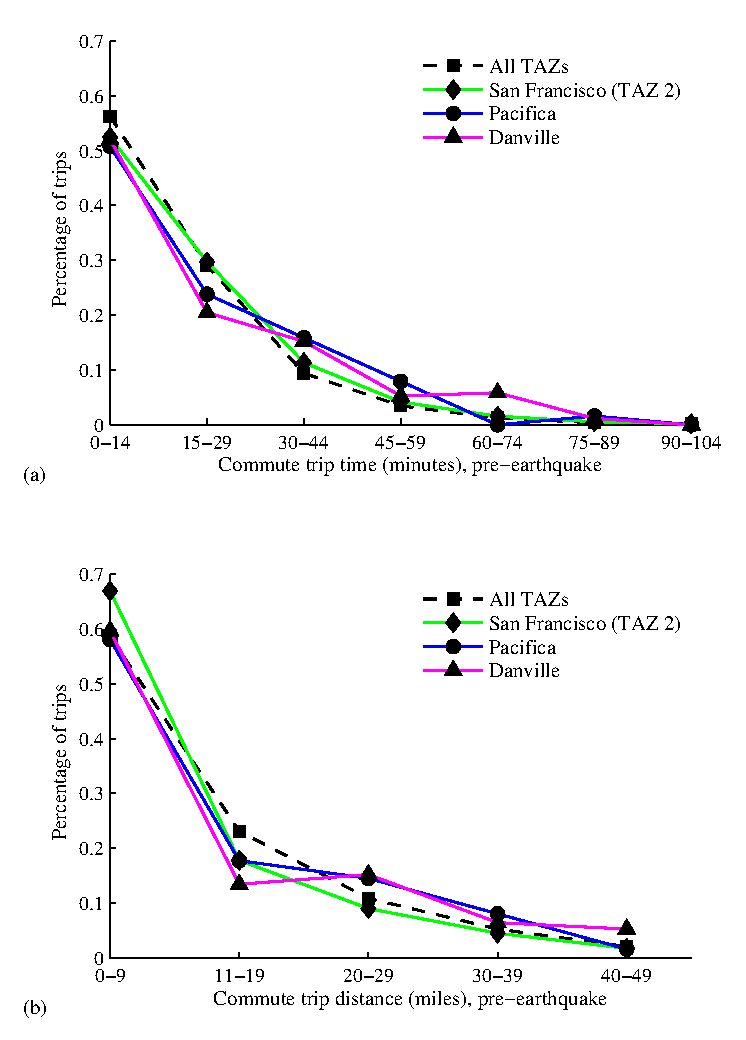
\includegraphics[width=4in]{FIGS/equity_trip_time_distance_pdfs_by_taz_to_work_and_from_work.eps} 
\caption{One-way commute trip information by (a) 15-minute time interval, and (b) 10-mile distance interval for 3 case study TAZs and the average over all TAZs.}
\label{fig:time_distance_pdfs}
\end{figure}



%\begin{figure}
%\centering
%\includegraphics[width=\textwidth]{../FIGS/equity_time_distance_SF.eps} 
%\caption{\textcolor{red}{TODO: add baseline, averaged over all TAZ?} Trip distributions for trips originating from San Francisco (TAZ 2)  after three earthquake events for a) trip length and b) trip time, as compared to the baseline.}
%\label{fig:time_distance_loss_sf}
%\end{figure}

%Third, as mentioned in the last section, areas away from the relatively more active Hayward and Calaveras faults in the East Bay have generally lower expected losses in accessibility. This is the case for this San Francisco TAZ. Specifically, the financial district is approximately 11 miles (18km) West of the closest segment of the Hayward Fault, with most areas even further away. Nonetheless, this is still close enough for some impact from these faults, e.g., as shown in Figure~\ref{fig:scen_acc}{(b)}. So, the results suggest that one factor to the relatively lower risk for San Francisco is being located on the San Francisco Peninsula (with a moderate separation distance from the East Bay faults), but not the key factor.
%%TODO: consider making a heat map of destinations from SF. Are they mostly avoiding East Bay bridges???

In summary, the data suggests that a major cause for the the low expected accessibility impact for the financial district of San Francisco is the lower relative dependence on cars for mobility. In the next section, we will contrast the San Francisco example with results from Pacifica, another Peninsula community that, nonetheless, is expected to be at high risk of losses in accessibility.